%%% License: Creative Commons Attribution Share Alike 4.0 (see https://creativecommons.org/licenses/by-sa/4.0/)


%%%%%%%%%%%%%%%%%%%%%%%%%%%%%%%%%%%%%%%%%

%----------------------------------------------------------------------------------------
%	PACKAGES AND OTHER DOCUMENT CONFIGURATIONS
%----------------------------------------------------------------------------------------

\documentclass[a4paper]{article}

\usepackage{amssymb}
\usepackage{enumerate}
\usepackage[usenames,dvipsnames]{color}
\usepackage{fancyhdr} % Required for custom headers
\usepackage{lastpage} % Required to determine the last page for the footer
\usepackage{extramarks} % Required for headers and footers
\usepackage[usenames,dvipsnames]{color} % Required for custom colors
\usepackage{graphicx} % Required to insert images
\usepackage{listings} % Required for insertion of code
\usepackage{courier} % Required for the courier font
\usepackage[table]{xcolor}
\usepackage{amsfonts,amsmath,amsthm,parskip,setspace,url}
\usepackage[section]{placeins}
\usepackage[a4paper]{geometry}
\usepackage[USenglish]{babel}
\usepackage[utf8]{inputenc}
\usepackage{tikz}


% Margins
\topmargin=-0.45in
\evensidemargin=0in
\oddsidemargin=0in
\textwidth=6.5in
\textheight=9.0in
\headsep=0.6in

\linespread{1.1} % Line spacing



%----------------------------------------------------------------------------------------
%   FORMATTING
%----------------------------------------------------------------------------------------
% Set up the header and footer
\pagestyle{fancy}
\lhead[c]{\textbf{{\color[rgb]{.5,0,0} K{\o}benhavns\\Universitet }}} % Top left header
\chead{\textbf{{\color[rgb]{.5,0,0} \Class }}\\ \hmwkTitle  } % Top center head
\rhead{\instructor \\ \theprofessor} % Top right header
\lfoot{\lastxmark} % Bottom left footer
\cfoot{} % Bottom center footer
\rfoot{Page\ \thepage\ of\ \protect\pageref{LastPage}} % Bottom right footer
\renewcommand\headrulewidth{0.4pt} % Size of the header rule
\renewcommand\footrulewidth{0.4pt} % Size of the footer rule


% Other formatting stuff
%\setlength\parindent{12pt}
\setlength{\parskip}{5 pt}
%\theoremstyle{definition} \newtheorem{ex}{\textbf{\Large{Exercise & #}\\}}
\usepackage{titlesec}
\titleformat{\section}[hang]{\normalfont\bfseries\Large}{Problem \thesection:}{0.5em}{}




%----------------------------------------------------------------------------------------
%	NAME AND CLASS SECTION
%----------------------------------------------------------------------------------------
\newcommand{\hmwkTitle}{Exercises for Lecture 6 (M2)} % Assignment title
\newcommand{\Class}{Mechanism Design} % Course/class
\newcommand{\instructor}{Fall 2021} % TA
\newcommand{\theprofessor}{Prof. Egor Starkov} % Professor




%----------------------------------------------------------------------------------------
%   SOLUTIONS
%----------------------------------------------------------------------------------------
\newif\ifsolutions
\solutionstrue




\begin{document}

\begin{center}
		\LARGE\textbf{Exercises for Lecture 6 (M2):\\ Monotonicity and implementability.}
\end{center}




%\section{Judicial design}
%
%	Revisit problem 3 in L3 homework. Can you solve it now without looking at the solutions?
%
%\ifsolutions
%\section*{Solution}
%	See solutions to L3 HW.
%\fi



\section{Sufficiency of monotonicity in Euclidean setting}

	Prove that in a Euclidean setting, if $k(\theta)$ is monotone (in the required direction) then there exist $t(\theta)$ s.t. $(k,t)$ is DSIC.\\
	\emph{Hint: use the recipe from the slides: use the envelope representation of payoffs to construct transfers, then show that the resulting mechanism is DSIC.}

\ifsolutions
\section*{Solution}

	By plugging the definition of $U_i(\theta)$ into the envelope representation
	\begin{equation*}
		U_i(\theta_i, \theta_{-i}) = U_i (\underline{\theta}_i,\theta_{-i}) + \int_{\underline{\theta}_i}^{\theta_i} k_i(s,\theta_{-i}) d s,
	\end{equation*}
	we can express the transfers in terms of allocation $k$ as
	\begin{align*}
		t_i(\theta_i,\theta_{-i}) = \theta_i k_i(\theta_i,\theta_{-i}) - U_i(\underline{\theta}_{i}, \theta_{-i}) - \int_{\underline{\theta}_{i}}^{\theta_i} k_{i} (s,\theta_{-i}) ds.
	\end{align*}
	Now consider a DRM given by the allocation $k$ fixed in the problem and transfers $t$ as defined above. We want to show this mechanism is DSIC. To do this, fix arbitrary $i,\theta_i,\hat{\theta}_i,\theta_{-i}$ and write out an IC constraint for $\theta_i$ to not be willing to misreport himself as $\hat{\theta}_i$:
	\begin{align}
		\theta_i k_i(\theta_i,\theta_{-i}) - t_i(\theta_i,\theta_{-i}) &\geq \theta_i k_i(\hat{\theta}_i,\theta_{-i}) - t_i(\hat{\theta_i},\theta_{-i})
		\nonumber
		\\ \iff
		U_i(\underline{\theta}_{i}, \theta_{-i}) + \int_{\underline{\theta}_{i}}^{\theta_i} k_{i} (s,\theta_{-i}) ds &\geq \left( \theta_i - \hat{\theta}_i \right) k_i(\hat{\theta}_i,\theta_{-i}) + U_i(\underline{\theta}_{i}, \theta_{-i}) + \int_{\underline{\theta}_{i}}^{\hat{\theta}_i} k_{i} (s,\theta_{-i}) ds.
		\label{eq:mon_IC}
	\end{align}
	If $\hat{\theta}_i < \theta_i$ then this reduces to
	\begin{align*}
		\int_{\hat{\theta}_{i}}^{\theta_i} k_{i} (s,\theta_{-i}) ds &\geq \left( \theta_i - \hat{\theta}_i \right) k_i(\hat{\theta}_i,\theta_{-i})
		\\ \iff
		\int_{\hat{\theta}_{i}}^{\theta_i} k_{i} (s,\theta_{-i}) ds &\geq \int_{\hat{\theta}_{i}}^{\theta_i} k_{i} (\hat{\theta}_i,\theta_{-i}) ds,
	\end{align*}
	which holds because by monotonicity ($k$ weakly increasing), $k_{i} (u,\theta_{-i}) \geq k_{i} (\hat{\theta}_i,\theta_{-i})$ for all $s \in [\hat{\theta}_i, \theta_i]$. For $\hat{\theta}_i > \theta_i$ inequality \eqref{eq:mon_IC} reduces to
	\begin{align*}
		\left( \hat{\theta}_i - \theta_i \right) k_i(\hat{\theta}_i,\theta_{-i}) & \geq \int_{\theta_{i}}^{\hat{\theta}_i} k_{i} (s,\theta_{-i}) ds,
	\end{align*}
	which holds by a mirror argument if $k$ is weakly increasing.
\fi



\section{Implementation in auctions}

	Consider the auction environment with two buyers.  Suppose that each buyer $i$ has willingness to pay $\theta_i$ drawn from the set $[0,1].$
	\begin{enumerate}
		\item Draw a square with $\theta_1$ on the horizontal axis and $\theta_2$ on the vertical axis.  A point in the square
		represents a profile $(\theta_1, \theta_2)$.
		\item Draw a downward sloping curve through the box.
		\item Draw an upward sloping curve through the box that intersects the downward sloping curve (exactly once.)
		\item The region above your downward sloping curve is divided into two subregions by your upward sloping curve.  Label
		the subregion that is above your upward sloping curve with a $2$ and label the other subregion with a $1$.  Label
		the entire region that is below (and to the left of) your downward sloping curve with a $0$.
		\item Consider the allocation rule that is defined by your drawing.  In the $1$ region agent $1$ gets the
		good, in the $2$ region agent $2$ gets the good and in the $0$ region neither agent gets the good.  (On the boundary
		between regions pick the allocation from one of the neighboring regions. )  Find a transfer rule which, when
		coupled with your allocation rule, forms a DSIC mechanism.
		
		\emph{Hint: you will probably need to use the envelope representation of payoffs that we obtained when deriving payoff-equivalence:}
		\begin{equation*}
			U_i(\theta_i, \theta_{-i}) = U_i (\underline{\theta}_i,\theta_{-i}) + \int_{\underline{\theta}_i}^{\theta_i} k_i(s,\theta_{-i}) d s
		\end{equation*}
		\emph{In particular, you can derive transfers that support $k$ using the expression above. But if you did Problem 3 above, you already know that.}
		
		\item Is there any DSIC allocation rule that picks alternatives from the set $\{0,1,2\}$ that could not be represented by a drawing that follows the instructions given above?
		\\
		(If not: argue verbally why not. If yes: draw a graph and argue intuitively why the $k$ you drew would be DSIC.)
	\end{enumerate}

\ifsolutions
\section*{Solution}

	\begin{figure}
	\begin{center} 
		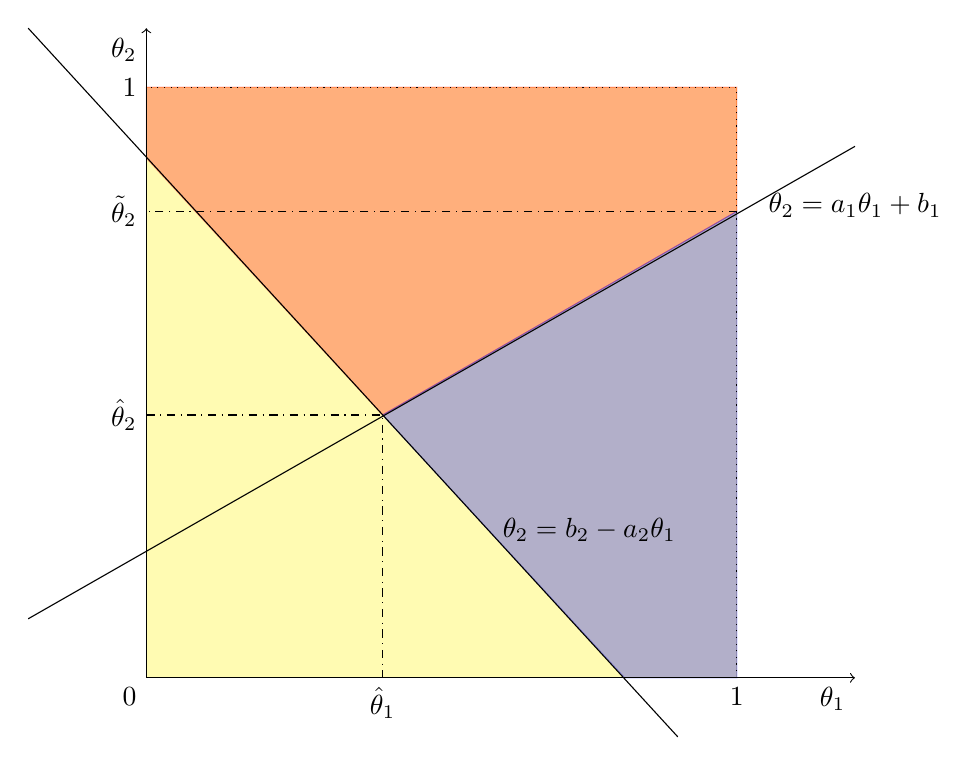
\begin{tikzpicture}[scale=7.5]
			%regions
			\filldraw[yellow, opacity=0.3] (0,0) -| (1,1) -| (0,0);
			\filldraw[red, opacity=0.3] (0,0.88) -- (0.4,0.445) -- (1,0.79) |- (0,1) -- (0,0.88);
			\filldraw[blue, opacity=0.3] (0.81,0) -- (0.4,0.445) -- (1,0.79) |- (0.81,0);
			
			% axes 
			\draw[->] (0,0) -- (1.2,0) node[below left]{$\theta_1$};
			\draw[->] (0,0) -- (0,1.1) node[below left]{$\theta_2$};
			\draw (0,0) node[below left]{$0$};
			\draw (0,1) node[left]{$1$};
			\draw (1,0) node[below]{$1$};
			
			% bounding box
			\draw[dotted] (1,0) |- (0,1);
			
			% two lines
			\draw (-0.2,0.1) -- (1.2,0.9);
			\draw (-0.2, 1.1) -- (0.9,-0.1);
			\draw (1.2,0.8) node {$\theta_2 = a_1 \theta_1 + b_1$};
			\draw (0.75,0.25) node {$\theta_2 = b_2 - a_2 \theta_1$};
			
			% special notation
			\draw[dashdotted] (1,0.79) -- +(-1,0) node[left]{$\tilde{\theta}_2$};
			\draw[dashdotted] (0,0.445) node[left]{$\hat{\theta}_2$} -| +(0.4,-0.445) node[below]{$\hat{\theta}_1$};
		\end{tikzpicture}
		\caption{an arbitrary allocation}
		\label{fig:2}
	\end{center}
	\end{figure}
	
	We will work with Figure \ref{fig:2}. Of course, there will be some things that are specific to the drawing, but the way we will solve the exercise should illustrate the general procedure for different figures.
	
	Based on the figure, we construct the following allocation:
	\begin{align*}
		k_1(\theta_1,\theta_2) &=
		\begin{cases}
			0 & \text{ if } \theta_2+a_2\theta_1\leq b_2\quad \text{ or }\quad \theta_2\geq b_1+a_1\theta_1\\
			1 & \text{otherwise}
		\end{cases}
		\\
		k_2(\theta_1,\theta_2) &=
		\begin{cases}
			0 & \text{ if } \theta_2+a_2\theta_1\leq b_2\quad \text{ or }\quad \theta_2\leq b_1+a_1\theta_1\\
			1 & \text{otherwise}
		\end{cases}
	\end{align*}
	
	We know that the allocation must be monotone for it to be implementable. However, it is very easy to check (just observe the drawing) that fixing the type of the other player, the probability of getting the good weakly increases with the player's type. Now we have to construct the transfers to implement this in dominant strategies. We will make use of the envelope representation of utility, mainly of the result that:
	\begin{align} \label{transfer}
		t_i(\theta_i,\theta_{-i}) = \theta_i k_i(\theta_i,\theta_{-i}) - U_i(\underline{\theta}_{i}) - \int_{\underline{\theta}_{i}}^{\theta_i} k_{i} (u,\theta_{-i}) du
	\end{align}
	are the transfers that work.
	
	Let's start with $t_1(\theta_1,\theta_2)$. Note that if $\theta_2>\tilde{\theta}_2$, then no matter what type player 1 announces, $k_1(\cdot,\theta_2)=0$. Hence, $t_1(\theta_1,\theta_2)=0$ for $\theta_2>\tilde{\theta}_2$. Consider now $\theta_2\in[\hat{\theta}_2,\tilde{\theta}_2]$. In that case, $k_1(\theta_1,\theta_2)=1$ if and only if $\theta_1\geq\frac{\theta_2-b_1}{a_1}$. Then for $\theta_2\in[\hat{\theta}_2,\tilde{\theta}_2]$:
	
	\[t_1(\theta_1,\theta_2)=\left\{\begin{array}{cc} 0 & \quad\text{ if }\quad  \theta_1\leq\frac{\theta_2-b_1}{a_1}\\
		\frac{\theta_2-b_1}{a_1} & \quad\text{otherwise}\quad
		
	\end{array}
	\right.
	\]
	where the last part comes from using (\ref{transfer}) and noticing that $\underline{\theta}_1=\frac{\theta_2-b_1}{a_1}$ and setting $U_1(\underline{\theta}_1)=0$:
	\begin{align*}
		t_1(\theta_1,\theta_2)=\theta_1-\int_{\frac{\theta_2-b_1}{a_1}}^{\theta_1}1 du=\frac{\theta_2-b_1}{a_1}
	\end{align*}
	Finally, consider $\theta_2\leq\hat{\theta}_2$. In that case, $k_1(\cdot,\theta_2)=0$ for $\theta_1\leq \frac{b_2-\theta_2}{a_2}=\underline{\theta}_1$. Then, in that case:
	
	\[t_1(\theta_1,\theta_2)=\left\{\begin{array}{cc} 0 & \quad\text{ if }\quad  \theta_1\leq\frac{b_2-\theta_2}{a_2}\\
		\frac{b_2-\theta_2}{a_2} & \quad\text{otherwise}\quad
		
	\end{array}
	\right.
	\]
	
	Notice that, apart from Problem 3 saying it is the case, it is clear why the mechanism is DSIC: whether the player pays or not depends on his announcement, but not how much he pays. In this sense, it is like a SPA.
	
	We can calculate the transfers for player 2 in a similar manner. Consider $\theta_1<\hat{\theta}_1$. Then, $k_2(\theta_1,\theta_2)=0$ if $\theta_2\leq b_2-a_2 \theta_1$. Then,
	
	\[t_2(\theta_1,\theta_2)=\left\{\begin{array}{cc} 0 & \quad\text{ if }\quad  \theta_2\leq b_2-a_2 \theta_1\\
		b_2-a_2 \theta_1 & \quad\text{otherwise}\quad
		
	\end{array}
	\right.
	\]
	On the other hand, if $\theta_1\geq\hat{\theta}_1$, we have that $k_2(\theta_1,\theta_2)=0$ if $\theta_2\leq a_1\theta_1+b_1$. Then:
	\[t_2(\theta_1,\theta_2)=\left\{\begin{array}{cc} 0 & \quad\text{ if }\quad  \theta_2\leq b_1+a_1 \theta_1\\
		b_1+a_1 \theta_1 & \quad\text{otherwise}\quad
		
	\end{array}
	\right.
	\]
	
	
	
	Now for the last part of the question: whether there exists a DSIC allocation rule that cannot be represented by a drawing described in the problem. The answer is yes, one example is as follows.
	Consider the allocation depicted in Figure \ref{fig:3}, which is given by (the exact numbers do not matter):
	\begin{align*}
		k(\theta_1,\theta_2) = \begin{cases}
			1 & \text{ if } \theta_1 \geq \max\{ 0.7 - \theta_2, \ 0.2 + \theta_2 \};
			\\
			2 & \text{ if } \theta_2 \geq \max\{ 0.7 - \theta_1, \ 0.2 + \theta_1 \};
			\\
			0 & \text{ otherwise.}
		\end{cases}
	\end{align*}
	
	This allocation is again monotone for each player ($k_i$ weakly increasing in $\theta_i$ given fixed $\theta_j$). We can construct the transfers that DSIC-implement it in the same way as we did in the main problem above (using \eqref{transfer}).
	
	\begin{figure}
		\centering
		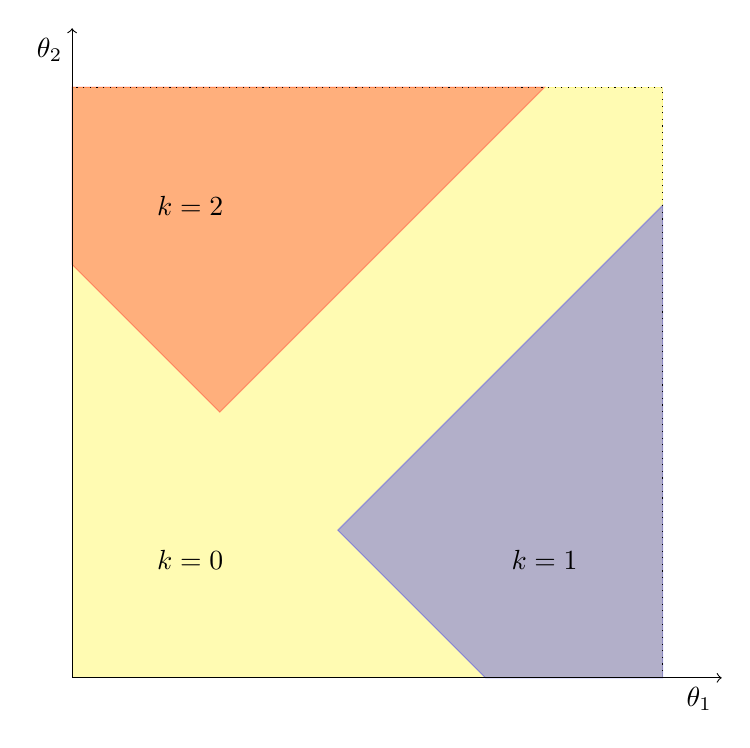
\begin{tikzpicture}[scale=7.5]
			\filldraw[yellow, opacity=0.3] (0,0) -| (1,1) -| (0,0);
			\filldraw[red, opacity=0.3] (0,0.7) -- (0.25,0.45) -- (0.8,1) -| (0,0.7);
			\filldraw[blue, opacity=0.3] (0.7,0) -- (0.45,0.25) -- (1,0.8) |- (0.7,0);
			
			\draw(0.2,0.2) node{$k=0$};
			\draw(0.2,0.8) node{$k=2$};
			\draw(0.8,0.2) node{$k=1$};
			
			% axes 
			\draw[->] (0,0) -- (1.1,0) node[below left]{$\theta_1$};
			\draw[->] (0,0) -- (0,1.1) node[below left]{$\theta_2$};
			
			% bounding box
			\draw[dotted] (1,0) |- (0,1);
		\end{tikzpicture}
		\caption{an even more arbitrary DSIC allocation} \label{fig:3}
	\end{figure}

\fi





%%-----------------------------------------------------------------------------------------------------

\end{document}
